\begin{figure*}[t]
    \centering

    \begin{subfigure}[b]{.23\textwidth}
        \centering
        \resizebox{\textwidth}{!}{\includegraphics{figure/plot/reference/fig2a-pointer-chasing.tikz.pdf}}
        \caption{\label{fig:2:ref:ptr-chasing-vanilla}[Ref] Pointer Chasing}
    \end{subfigure}
    \hfill
    \begin{subfigure}[b]{.23\textwidth}
        \centering
        \resizebox{\textwidth}{!}{
        \scriptsize \bfseries \ttfamily
            \begin{tabular}{|r|r|r|r|} \hline
            \multicolumn{1}{|c|}{PC-Block} & \multicolumn{1}{c|}{L1 NVC} & \multicolumn{1}{c|}{L2 NVC} & \multicolumn{1}{c|}{WPQ} \\ \hline
            64B                            & 1.84                        & 1.18                        & 3.78                     \\ \hline
            256B                           & 1.00                        & 1.17                        & 1.07                     \\ \hline
            512B                           & \cellcolor{blue!25}1.00     & 1.11                        & \cellcolor{blue!25}1     \\ \hline
            1K                             & 0.99                        & 1.07                        & 1                        \\ \hline
            2K                             & 0.97                        & 1.03                        & 1                        \\ \hline
            4K                             & 0.96                        & \cellcolor{blue!25}1.00     & 1                        \\ \hline
            \end{tabular}
        }
        \captionsetup{skip=10pt}
        \caption{\label{fig:2:ref:ptr-chasing-amplification}[Ref] Amplification}
    \end{subfigure}
    \hfill
    \begin{subfigure}[b]{.23\textwidth}
        \centering
        % \resizebox{\textwidth}{!}{\includegraphics{figure/plot/reproduce/fig2a-pointer-chasing.tikz.pdf}}
        \resizebox{\textwidth}{!}{\includegraphics{example-image-duck}}
        \caption{\label{fig:2:rep:ptr-chasing-vanilla}[Rep] Pointer Chasing}
    \end{subfigure}
    \hfill
    \begin{subfigure}[b]{.23\textwidth}
        \centering
        \resizebox{\textwidth}{!}{
        \scriptsize \bfseries \ttfamily
            \begin{tabular}{|r|r|r|r|} \hline
            \multicolumn{1}{|c|}{PC-Block} & \multicolumn{1}{c|}{L1 NVC} & \multicolumn{1}{c|}{L2 NVC} & \multicolumn{1}{c|}{WPQ} \\ \hline
            64B                            &                             &                             &                          \\ \hline
            256B                           &                             &                             &                          \\ \hline
            512B                           &                             &                             &                          \\ \hline
            1K                             &                             &                             &                          \\ \hline
            2K                             &                             &                             &                          \\ \hline
            4K                             &                             &                             &                          \\ \hline
            \end{tabular}
        }
        \captionsetup{skip=10pt}
        \caption{\label{fig:2:rep:ptr-chasing-amplification}[Rep] Amplification}
    \end{subfigure}

    \caption{\label{fig:2}Pointer chasing microbenchmark results and amplification factors for each architectural components.}

\end{figure*}
